% !TeX spellcheck = cs_CZ
\documentclass[a4paper,hidelinks]{report}

\usepackage[utf8]{inputenc}
\usepackage[czech]{babel}
\usepackage{hyperref}
\usepackage{amsmath}
\usepackage{amsfonts}
\usepackage{amssymb}
\usepackage{listingsutf8}
\usepackage[table]{xcolor}
\usepackage{inconsolata}
\usepackage{nameref}
\usepackage{pifont}
\usepackage{placeins}
\usepackage[a4paper,includeheadfoot,margin=3.5cm]{geometry}
\usepackage{multirow}
\usepackage{pdflscape}
\newcommand{\cmark}{\ding{51}}
\newcommand{\xmark}{\ding{55}}

%Vkladani source kodu
\lstdefinestyle{codeInput} { %
	language=C++,
	basicstyle=\ttfamily\footnotesize,
	numberstyle=\scriptsize,
	numbers=left,
	backgroundcolor=\color{gray!10},
	frame=single,
	keepspaces=true,  
	showspaces=false,
	showstringspaces=false,
	showtabs=false,
	tabsize=4,
	rulecolor=\color{black!30},
	escapeinside={\%*}{*)},
	breaklines=true,
	breakatwhitespace=true,
	framextopmargin=2pt,
	framexbottommargin=2pt,
	inputencoding=utf8/latin2,
	extendedchars=true,
	literate=
	{á}{{\'a}}1
	{í}{{\'i}}1
	{é}{{\'e}}1
	{ý}{{\'y}}1
	{ú}{{\'u}}1
	{ó}{{\'o}}1
	{ě}{{\v{e}}}1
	{š}{{\v{s}}}1
	{č}{{\v{c}}}1
	{ř}{{\v{r}}}1
	{ž}{{z}}1
	{ď}{{\v{d}}}1
	{ť}{{\v{t}}}1
	{ň}{{\v{n}}}1                
	{ů}{{\r{u}}}1
	{Á}{{\'A}}1
	{Í}{{\'I}}1
	{É}{{\'E}}1
	{Ý}{{\'Y}}1
	{Ú}{{\'U}}1
	{Ó}{{\'O}}1
	{Ě}{{\v{E}}}1
	{Š}{{\v{S}}}1
	{Č}{{\v{C}}}1
	{Ř}{{\v{R}}}1
	{Ž}{{\v{Z}}}1
	{Ď}{{\v{D}}}1
	{Ť}{{\v{T}}}1
	{Ň}{{\v{N}}}1                
	{Ů}{{\r{U}}}1    	
}
\lstset{style=codeInput}
\renewcommand{\lstlistingname}{Zdrojový kód}
\renewcommand{\lstlistlistingname}{Seznam zdrojových kódů}
\newcommand{\includecode}[3][default]
{\lstinputlisting[caption=#3,label=lst:#1, style=codeInput]{#2}}


\title{Simulace Sluneční soustavy}
\date{\today}
\author{Jan Waltl}


\usepackage{graphicx}
\DeclareGraphicsExtensions{.pdf,.png,.jpg}
\usepackage{fancyhdr}
\setlength{\headheight}{15pt}

\pagestyle{fancy}
\renewcommand{\chaptermark}[1]{ \markboth{\thechapter \ #1}{} }
\renewcommand{\sectionmark}[1]{ \markright{\thesection \ #1} }

\fancyhf{}
\fancyfoot[C]{\thepage}
\fancyhead[L]{\textit{ \expandafter\MakeUppercase\expandafter{\leftmark}} }
\fancyhead[R]{\textit{ {\rightmark}} }

\fancypagestyle{plain}{ %
	\fancyhf{} % remove everything
	\fancyfoot[C]{\thepage}
	\renewcommand{\headrulewidth}{0pt} % remove lines as well
	\renewcommand{\footrulewidth}{0pt}
}

\begin{document}
	\begin{titlepage}
	\begin{center}
		\vspace*{8cm}
		\Huge{\textbf{Simulace Sluneční soustavy}}\\
		\vspace*{1cm}
		{\Large Dokumentace k zápočtovému programu pro předmět Programování I}\\
		\vfill
		
		\huge{Jan Waltl}\\
		\huge{12.Ledna 2017}
	\end{center}
\end{titlepage}
	

	\pagenumbering{gobble}
	\newpage
	
	\tableofcontents
	\newpage
	% !TeX spellcheck = cs_CZ

\chapter*{Organizace dokumentu}
Tento text je organizován do následujících kapitol:
\begin{description}
	\item[\nameref{chap:uvod}] - Zadání zápočtového programu a teoretická část
	\item[\nameref{chap:implementace}] - Hlavní část dokumentace, které popisuje jak design celého programu, tak jednotlivých částí. Zaměřuje se na použité algoritmy a jejich implementaci včetně zdrojových kódů C++.
	Také zmiňuje možnosti rozšíření programu.
	\item[\nameref{chap:userGuide}] - Část popisující jak program spustit a jak s ním pracovat z neprogramátorského pohledu.
	
\end{description}
Text není nutné číst od začátku do konce, pro první spuštění by mělo stačit poslední kapitolu. Naopak, ale pro pochopení implementace RK4 metody je dobré vědět něco o numerické integraci a o co se vlastně program vůbec snaží. Což popisuje teoritická část v úvodní kapitole. Programátorská část vyžaduje znalost C++ a OpenGL, ale je zde snaha důležitější koncepty vysvětlit  i bez těchto znalostí. V tomto textu se nachází  zdrojové kódy s příklady, které jsou psány následujícím formátem:
\begin{lstlisting}
\caption{Text vystihující příklad (Název souboru)}
#include <iostream>

int main()
{
	std::cout<<"Hello World!\n";
	return 0;
}
\end{lstlisting}
Všechny další uvedené zdrojové kódy se nachází ve složce \texttt{Source/}, která
by měla být připojena k této dokumentaci. Z praktických důvodů \textbf{nemusí} být tyto soubory zkompilovatelné, popřípadě mohou být z části v pseudo-kódu. Také se \textbf{nejedná} o zdrojové kódy samotného programu. Primární účel je \textbf{popisný}. Ovšem často bude uvedený kód přímo nebo částečně odpovídat kódu někde uvnitř programu.
Zdrojové kódy samotného programu se přímo v tomto dokumentu nenachází, avšak jsou také součástí dokumentace a obsahují komentáře, které mohou stát za přečtení.
\vfill
\begin{center}
\textbf{	
Tato dokumentace spolu se zdrojovými kódy programu je dostupná na:\\
\texttt{https://bitbucket.org/Quimby/solar/src}\\
Popřípadě přímo stažitelná pomocí git:	\\
\texttt{https://Quimby@bitbucket.org/Quimby/solar.git}\\
V případě problému mne můžete kontaktovat na adrese: waltl.jan@gmail.com
}
\end{center}

	\pagenumbering{arabic}
	
	% !TeX spellcheck = cs_CZ

\chapter{Návrh programu}
\label{chap:implementace}
Tato kapitola se zabývá návrhem programu - jak je celý program navržen a popisuje jeho hlavní třídu - \texttt{Simulation}. V rámci které si představíme \textbf{moduly}, které se objevují v dalších kapitolách.
Na úvod se podívejme jak by mohl vypadat jednoduchý \textbf{main.cpp} 

\includecode{Source/main.cpp}{Hlavní program}

Veškeré zdrojové kódy programu jsou zabaleny do jmenného prostoru \texttt{solar}. \texttt{Simulation} je hlavní třída, která se stará o celkový průběh simulace. Dále jsou zde vidět tři \textbf{moduly}, které jsou předány simulaci. Jejich detailní popis přijde později.

\texttt{Simulation} poté zajišťuje jejich vzájemnou spolupráci. Metoda \texttt{Simulation::Start()} následně spustí samotnou simulaci podle předepsaných parametrů.
Pokud někde nastane chyba, dojde k vyvolání výjimky v podobě třídy \texttt{solar::Exception}, popřípadě jiných výjimek z rodiny \texttt{std::exception}.


% !TeX spellcheck = cs_CZ

\section{Třída \texttt{Simulation}}
Je třída, která spojuje jednotlivé moduly do funkčního celku a zajišťuje průběh celé simulace, proto stojí za to se na ni podrobněji podívat. Nejprve se podíváme na veřejné rozhraní, které dovoluje simulaci ovládat. Poté nahlédneme i dovnitř abychom zjistili jak to celé funguje.
\subsection{Veřejné rozhraní}
Přibližně takto vypadají veřejné metody třídy \texttt{Simulation} :
\includecode{Source/simPublic.cpp}{Veřejně rozhraní \texttt{Simulation}}
\paragraph{Řídící funkce}
jsou funkce, které řídí spuštěnou simulaci. Jsou volány z modulů, ne z hlavního programu. Většinou se jedná o jednoduché funkce na 1-2 řádky, proto zde nejsou jednotlivě popsány, ale z jejich názvů je zřejmé co dělají. Případný náhled do zdrojových kódů by to měl objasnit.
\paragraph{Konstruktor}
očekává 3 moduly, které se budou v simulaci používat, podrobněji se na ně podíváme za okamžik. Zde jim také předá odkaz na simulovaná data.
\paragraph{Metoda \texttt{Start()}}
provádí samotnou simulaci. V této metodě stráví program většinu času, popíšeme ji podrobně v sekci \ref{sec:startMetoda} - vysvětlíme její teoretický návrh a implementaci, což také objasní její parametry.
\subsection{Moduly}
\label{sub:moduly}
Nyní si vysvětlíme co to \textbf{moduly} jsou a k čemu slouží.
Zkusme se zaměřit co by měla každá simulace vlastně udělat:
\begin{enumerate}
	\item \textbf{Načíst data}, bez nich není co simulovat. Což se dá popsat dvěma slovy a implementovat stovky způsoby. Takže by stálo za to, aby simulace uměla všechny.
	\item \textbf{Simulovat data}. Z teorie už víme, že také neexistuje pouze jedna integrační metoda, takže bychom chtěli mít na výběr. Určitě totiž není moc šťastné řešení zvolit jednu metodu a doufat, že bude stačit na všechny simulace.
	\item \textbf{Uložit data}. Také se chceme našimi výsledky pochlubit, ale kdyby nám je simulace pracně získala a hned zahodila, tak to půjde těžko. Ovšem stálo by za to umět je ukládat v různých formátech nebo třeba rovnou odeslat někam po internetu.
	\item \textbf{Prohlížet data}. Představme si situaci: 3:38 ráno, naše značně vylepšená verze simulace právě doběhla. Přidali jsme do ní nově objevené asteroidy u kterých chceme spočítat trajektorie. Z hrůzou ale zjistíme, že Země není tam kde má být, dokonce tam není vůbec! Co se mohlo asi stát? To je dobrá otázka, proto by mohlo být dobré mít přístup k datům i během simulace a třeba si je někam průběžně ukládat.
\end{enumerate}
Teď už víme, co by měla každá simulace zvládnout, ale je vidět, že toho má umět celkem hodně a ještě různými způsoby. Nejlepší tedy bude, aby se simulace(ve formě třídy \texttt{Simulation}) opravdu starala jen o to, aby tyto kroky proběhly, ale to jak přesně proběhnou přenecháme někomu jinému -\textbf{ modulům}, které se vyskytují ve 3 druzích:
\begin{description}
	\item[parser] obstarává výrobu vstupních dat. Také na konci simulace může výsledná data uložit.
	\item[simMethod] provádí simulaci dat např. pomocí nějaké numerické metody.
	\item[viewer] má přístup k datům za běhu simulace a může je např. zobrazovat na obrazovku nebo ukládat stranou.
\end{description}
Práci jsme rozdělili, simulace by to celé měla tedy organizovat, což se děje právě pomocí metody \texttt{Start()}, tak si ji pojďme představit.
\subsection{Návrh metody \texttt{Start()}}
\label{sec:startMetoda}
Takto nějak by mohla vypadat na první pohled rozumná implementace:
\includecode[startPseudo]{Source/startPseudo.cpp}{Návrh metody \texttt{Start()}}
Tato implementace by byla plně funkční, ale možná ne úplně vhodná pro náš cíl. Rádi bychom totiž prováděli a hlavně zobrazovali simulaci v reálném čase. 

Zde ale není žádné časování, \texttt{while} smyčka bude probíhat jak nejrychleji může, bez jakékoliv kontroly. Což není špatné, pokud chceme nechat program běžet a jen se pak podívat na výsledky, popřípadě mezivýsledky uložené někde v souborech. K tomu přesně slouží metoda \texttt{Simulation::StartNotTimed()}, která má přibližně výše uvedenou implementaci. 
\paragraph{Časování}
- K dosažení našeho cíle bude potřeba nějakým způsobem svázat reálný čas s tím simulovaným. Upravíme tedy předchozí příklad \ref{lst:startPseudo} následovně:
\includecode[startTimed]{Source/startPseudoTimed.cpp}
{Metoda \texttt{Start()} s časováním}
Pokud bychom chtěli opravdu simulaci v reálném čase, tak se v každém průběhu smyčkou podíváme jak dlouho trvala předchozí smyčka a tolik času musíme odsimulovat. Naivní implementace by byla předat přímo tento čas \texttt{acc} metodě, která se stará o simulaci. Tím bychom dostali nedeterministický algoritmus
\footnote{Algoritmus, který nemusí nutně vracet stejný výsledek při opakovaném volání se stejnými vstupními hodnotami.}.
Neboť trvání poslední smyčky je ovlivněno např. aktuálním vytížením počítače, což určitě není předvídatelné. A bohužel při počítaní s desetinnými čísly dochází k zaokrouhlovacím chybám, takže výsledek nezávisí pouze na vstupních datech, ale i na postupu výpočtu.

Řešení \footnote{Zdroj: \url{http://gafferongames.com/game-physics/fix-your-timestep/} (\today)}
je naštěstí jednoduché, budeme odečítat pevnou hodnotu \texttt{deltaT}.
A to tolikrát, abychom odsimulovali potřebný čas uložený v \texttt{acc}. Je pravda,
že nakonci nemusí platit $ acc=0 $, ale bude platit $ acc\leq deltaT $. A vzhledem k tomu, že \texttt{acc} si zachovává hodnotu mezi průběhy smyčkou, tak se zbytek času neztrácí, ale použije se v dalším průchodu. Takto dostaneme deterministický algoritmus.

\label{par:spiral}
Navíc máme objasněn první parametr - \textbf{deltaT(dt)} - základní časový krok simulace, který odpovídá $ \Delta t $ z teorie. Čím menší, tím je simulace přesnější, ale dochází k více voláním simulační metody, což může být potencionálně náročné na CPU.
Pro nízké hodnoty by se klidně mohlo snadno stát, že simulace přestane stíhat, tzn. že simulovat čas \texttt{deltaT} bude reálně trvat déle než \texttt{deltaT}. Např.
simulace \texttt{10ms} bude konstantně trvat \texttt{15ms}, v dalším průběhu smyčkou se tedy bude simulace snažit simulovat uběhlých \texttt{15ms}, což ale může trvat \texttt{22,5ms}. V dalším průběhu se tedy musí odsimulovat \texttt{22,5ms}...takový případ velmi rychle celý program odrovná. Proto je vhodné proměnnou \texttt{acc} omezit nějakou konstantou. Poté sice začne docházet ke zpožďování simulace, ale kontrolovaným způsobem.
\paragraph{Změna rychlosti} - Nyní bude naše simulace fungovat zcela správně a v reálném čase. Takže máme hotovo? Skoro, naše simulace je sice plně funkční, ale jediné co umí je předpovídat přítomnost a ještě jen s omezenou přesností. To není moc užitečné. Oběh Země kolem Slunce bude skutečně trvat 1 rok a Neptun to zvládne za 165 let. Tolik času nejspíše nemáme, proto by stálo za to najít nějaký způsob jak simulaci urychlit. Existují dva způsoby jak to udělat:
\begin{enumerate}
	\item Volat simulační metodu častěji. Například pro každý krok \texttt{deltaT} ji můžeme zavolat \texttt{rawMult}krát. Toto zrychlení jde na úkor výpočetního výkonu nutného k udržení této rychlosti, viz. předchozí odstavec.
	\item Volat simulační metodu s jiným \texttt{deltaT}, konkrétně s jeho \texttt{DTMult} násobkem. Tohoto zrychlení dosáhneme na úkor přesnosti. Protože předáváme větší $ \Delta t $ do simulační metody, což vede k menší přesnosti.
\end{enumerate}
Parametry \texttt{rawMult} a \texttt{DTMult} přesně odpovídají argumentům implementované verze metody \texttt{Simulation::Start()}.

Poslední parametr, který nebyl ještě vysvětlen je \texttt{maxSimTime}. Vzhledem k tomu, že volání funkce \texttt{Start()} může trvat velmi dlouho, tak je dobré nastavit horní limit, který garantuje přerušení smyčky po překročení zadaného času. \texttt{maxSimTime=0} znamená \texttt{maxSimTime=$ \infty $} ,tzn. simulace se přeruší pouze zavoláním funkce \texttt{Simulation::StopSimulation()}, kterou ale mohou volat pouze moduly, neboť jiné objekty nejsou při simulaci volány.
Popřípadě se přeruší vyvoláním nějaké vyjímky.

\subsection{Finální implementace metody \texttt{Start()}}
Poučeni z předchozí části upravíme naši rozpracovanou implementaci \ref{lst:startTimed} na \ref{lst:startFinal}. Což je už velmi podobné skutečné metodě použité v programu. Která navíc umožňuje simulaci pozastavit, krokovat a také pomocí C++ knihovny \texttt{chrono} implementuje opravdové časování, které zde bylo uvedeno spíše koncepčně.
\includecode[startFinal]{Source/startFinal.cpp}
{Finální verze \texttt{Simulation::Start()}}



\section{Výjimky}
Existují tři druhy výjimek, které program může vyvolat.
\begin{enumerate}
	\item Nejčastěji to bude výjimka v podobě třídy \texttt{Exception}, která dědí 
	z \texttt{std::runtime\_error} a tedy i \texttt{std::exception}. K této výjimce dojde zejména při chybě v otevírání/čtení souborů a inicializace knihoven, ale jedná se o hlavní třídu výjimek v tomto programu, takže je použita i v modulech pro hlášení chyb.
	\item Na výjimku v podobě třídy \texttt{GLError} můžeme narazit při chybě týkající se OpenGL - nepodařená inicializace, nedostatek paměti a podobně.
\item Výjimky dědící z \texttt{std::exception} - program využívá standardní C++ knihovny, které můžou potencionálně také vyvolat výjímky.
\end{enumerate}
Všechny tři druhy nabízí metodu \texttt{what()}, která vrátí krátký popis vyvolané výjimky.
	\chapter{Uživatelská příručka}
\label{chap:userGuide}
\section{Požadavky}
Vyžaduje verzi OpenGL 3 nebo vyšší, navíc je potřeba balíček Microsoft Visual C++ 2015 Redistributable, který je ve formě .dll přibalen. Pokud by s ním přesto byly problémy, tak doporučuji stáhnout  a nainstalovat jeho aktuální verzi z \url{https://www.microsoft.com/cs-CZ/download/details.aspx?id=53840}
\section{Základní ovladání}
Při spuštění se program otevře v výchozím grafickém režimu, kde dojde k nahrání zabudované Sluneční soustavy. Simulace se ovládá pomocí grafického rozhraní - Obrázek \ref{fig:GUI1}.\\
\begin{figure}
	\caption{Grafické rozhraní programu}
	\label{fig:GUI1} 
	\centering
	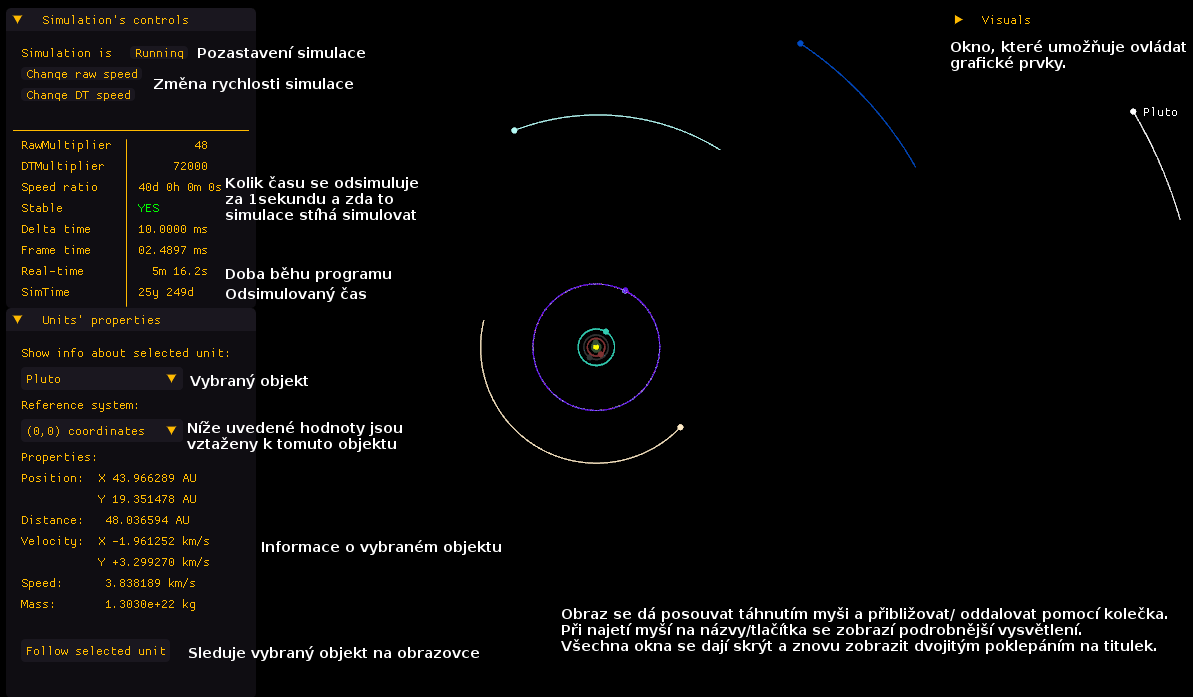
\includegraphics[scale=0.5]{Figs/GUI1_edited}
\end{figure}
\FloatBarrier
\section{Pokročilé možnosti}
Program také nabízí pokročilejší ovládání pomocí příkazové řádky, s níž je možné načítat simulovaná data ze souboru, vybrat si integrační metody a také možnost zaznamenat a následně přehrát uložené simulace.
Pro vypsání nápovědy a všech dostupných příkazů v českém jazyce použijte:
\ \texttt{\textbf{SolarSystem.exe -help -cz}}
\\\\
Uveďme zde alespoň pár dalších příkladů různých příkazů:
\begin{enumerate}
	\item \texttt{\textbf{SolarSystem.exe vstup.txt}} \\
	Načte vstupní data z formátovaného souboru \texttt{vstup.txt} a spustí simulaci, která bude běžet v reálném čase a zobrazovat se v okně 1200x700 s uživatelským rozhraním.
	\item \texttt{\textbf{SolarSystem.exe -sim -p formatted -i vstup.txt -m RK4 -v win}} \\
	 Ekvivalentní zápis předchozího příkladu. S explicitním použitím modulů.
	\item \texttt{\textbf{SolarSystem.exe -sim -rm 24 -dm 3600 -x 300}} \\
	Spustí podobnou simulaci jako v 1. příkladu. Akorát bude mít 3600x větší integrační krok a bude probíhat 10x rychleji. Ve výsledku se tedy odsimuluje jeden den za jednu reálnou sekundu. Simulace se vypne po 5 minutách běhu.
	\item \texttt{\textbf{SolarSystem.exe -record -r zaznam.replay -p formatted -i vstup.txt -o vystup.txt -m semiEuler -rm 24 -dm 3600 -x 60}}\\
	Zaznamená 60 sekundovou simulaci do souboru \texttt{zaznam.replay}, vstupní data načte z formátovaného souboru \texttt{vstup.txt} a výsledná data uloží do \texttt{vystup.txt} ve stejném formátu. Simulace bude simulovat jeden den za jednu sekundu pomocí semi-implicitní Eulerovy integrační metody. Simulace se spustí v grafickém prostředí stejně jako v 1. příkladě.
	\item  \texttt{\textbf{SolarSystem.exe zaznam.replay}}\\
	Přehraje zaznamenanou simulaci z předchozího příkladu v grafickém prostředí.
\end{enumerate}
K .exe souboru je přiložen vzorový formátovaný text \texttt{vstup.txt} a také jeden záznam simulace \texttt{zaznam.replay}.
Přesný popis formátovaného vstupního souboru je uveden v sekci \ref{sec:strukturaDat} . Pro detailní vysvětlení parametrů simulace je k dispozici popis v sekci \ref{sec:startMetoda}.


\chapter{Kompilace programu}
\label{chap:kompilace}
\section{Git}
Tato dokumentace spolu se zdrojovými kódy programu je veřejně dostupná na:
\begin{center}
\texttt{https://bitbucket.org/Quimby/solar/src}
\end{center}
Popřípadě přímo stažitelná pomocí git HTTPS\eqref{git:https} nebo SSH\eqref{git:ssh}:
\begin{align}
	\label{git:https}
	\texttt{https://Quimby@bitbucket.org/Quimby/solar.git}\\
	\label{git:ssh}
	\texttt{git@bitbucket.org:Quimby/solar.git}
\end{align}
\section{Windows}
Program byl tvořen v programu Visual Studio 2015 Community Edition, takže je zde už předpřipravený .sln projekt, který by měl obsahovat vše potřebné pro správné zkompilování.
\section{Linux}
Program by zde měl být teoreticky také plně funkční, avšak není zde zatím žádný pomocný projekt ani makefile. Kdyžtak je potřeba nejdříve stáhnout a zkompilovat externí knihovny - GLFW, GLEW. Návod by měl být na jejich oficiálních stránkách . Momentálně obě knihovny nabízí vytvoření potřebných souborů pomocí programu CMake, takže kompilace by neměla být těžká. Dále kompilace samotného programu vyžaduje minimálně flag \texttt{GLEW\_STATIC} a také include path do složky obsahující složku \texttt{Source/}(defaultně se nachází ve složce SolarSystem) a samozřejmě slinkovat obě knihovny, ale pak by už mělo vše fungovat. 
	 \begin{thebibliography}{1}
		\bibitem{projMatice}  Song Ho Ahn - { \em OpenGL Projection Matrix}\\ \url{http://www.songho.ca/opengl/gl_projectionmatrix.html}
		
		\bibitem{rotMatice}  Glen Murray - {\em Rotation About an Arbitrary Axis in 3 Dimensions} , 6.června 2013\\
		\url{https://sites.google.com/site/glennmurray/Home/rotation-matrices-and-formulas}
		
		\bibitem{ostatniMatice} Joey De Vries - {\em Úvod k maticím a vektorům}
		\url{https://learnopengl.com/#!Getting-started/Transformations}
		\bibitem{coords} Joey De Vries - {\em Coordinate Systems}\\
		\url{https://learnopengl.com/#!Getting-started/Coordinate-Systems}
		\bibitem{lookAt} Joey De Vries - {\em LookAt matice}\\
		\url{https://learnopengl.com/#!Getting-started/Camera}
		
		\bibitem{depthBuff} Joey De Vries - {\em Depth buffer}\\
		\url{https://learnopengl.com/#!Advanced-OpenGL/Depth-testing}
		\bibitem{logBuff}  Brano Kemen - {\em Maximizing Depth Buffer Range and Precision}\\
		\url{http://outerra.blogspot.cz/2012/11/maximizing-depth-buffer-range-and.html}
		\bibitem{revBuff} theo -  { \em Depth Precision}\\
		\url{http://dev.theomader.com/depth-precision/}
		\bibitem{GLEXT} Podpora OpenGL rozšíření u ruzných GPU\\
		\url{http://opengl.gpuinfo.org/gl\_extensions.php}
		\bibitem{srovnaniBuffer} Interaktivní srovnání logaritmického a klasického depth bufferu\\
		\url{baicoianu.com/~bai/three.js/examples/webgl_camera_logarithmicdepthbuffer.html}
		\bibitem{implRevBuff} Implementace reversed depth bufferu pro OpenGL\\
		\url{https://nlguillemot.wordpress.com/2016/12/07/reversed-z-in-opengl/}
		\bibitem{floatBlog} Bruce Dawson - { \em Blog s výbornými články o problematice floating-point čísel}\\
		\url{https://randomascii.wordpress.com/2012/02/13/dont-store-that-in-a-float/}
		\bibitem{GLFW} GLFW - dokumentace ke kompilaci knihovny
		\url{http://www.glfw.org/docs/latest/compile_guide.html}
	\end{thebibliography}
\end{document}
